% Team 8 evidence regenerated by the unified branch. Parameters: data/processed/
% team8/calibration_q040_audited_20261024/*.json; price/IV errors: Article 8
% img/diagnostics_ibkr/model_error_summary.csv (same q=0.40% calibration).

\subsubsection{Regenerated market-input and return evidence}

The scalar calibration errors reported above are interpretable only together
with the empirical objects that generated them. Figure~\ref{fig:t8-market-inputs}
shows the dated Treasury proxy and the structured option sample rebuilt by the
unified branch from the 2 September 2026 Team 8 snapshot. The raw licensed rows
remain local and Git-ignored; the figures and aggregate calibration outputs
carry hashes in the code-run manifest.

\begin{figure}[H]
    \centering
    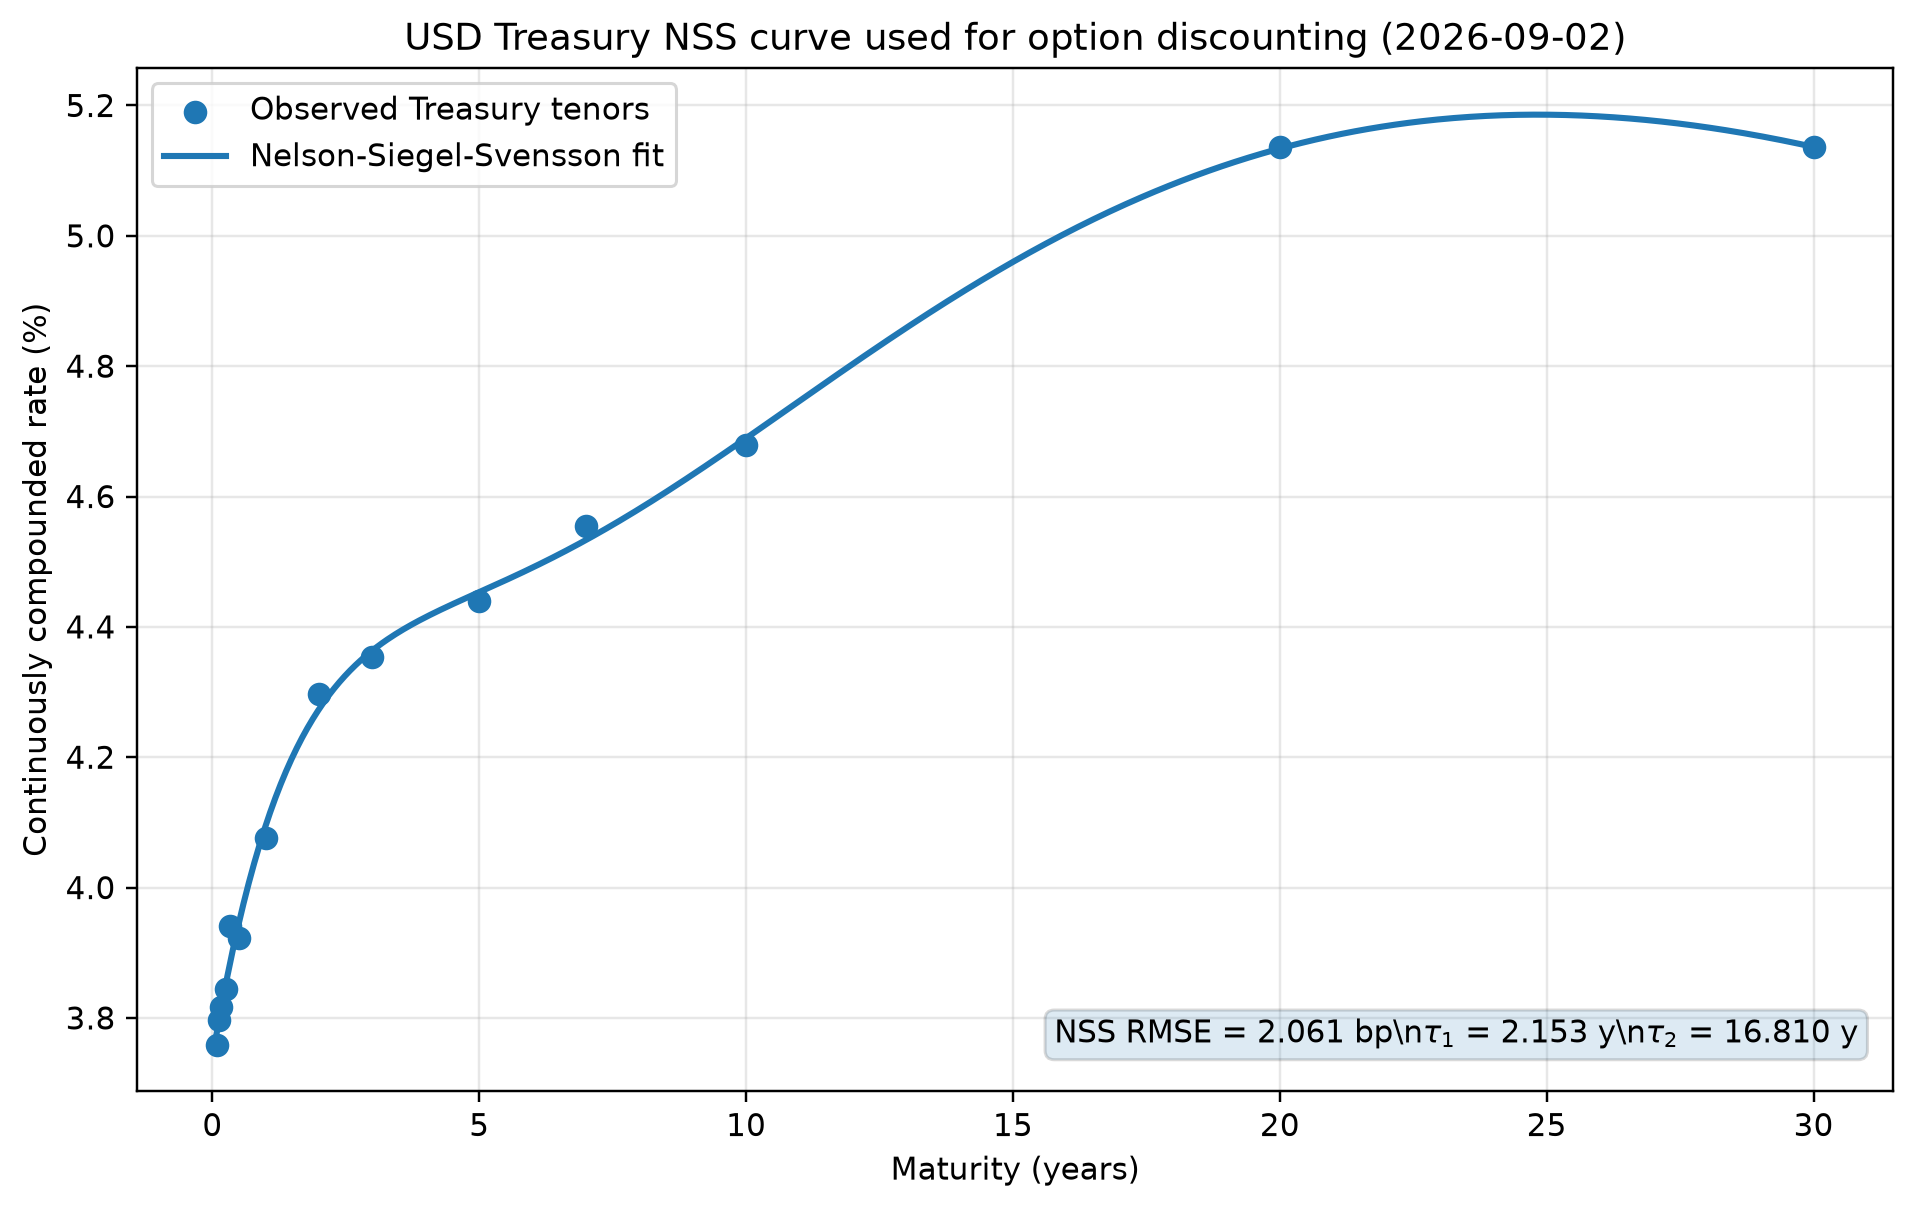
\includegraphics[width=0.82\textwidth]{../img/publication/f751012d2636c3b8_usd_treasury_curve.png}

    \vspace{4mm}
    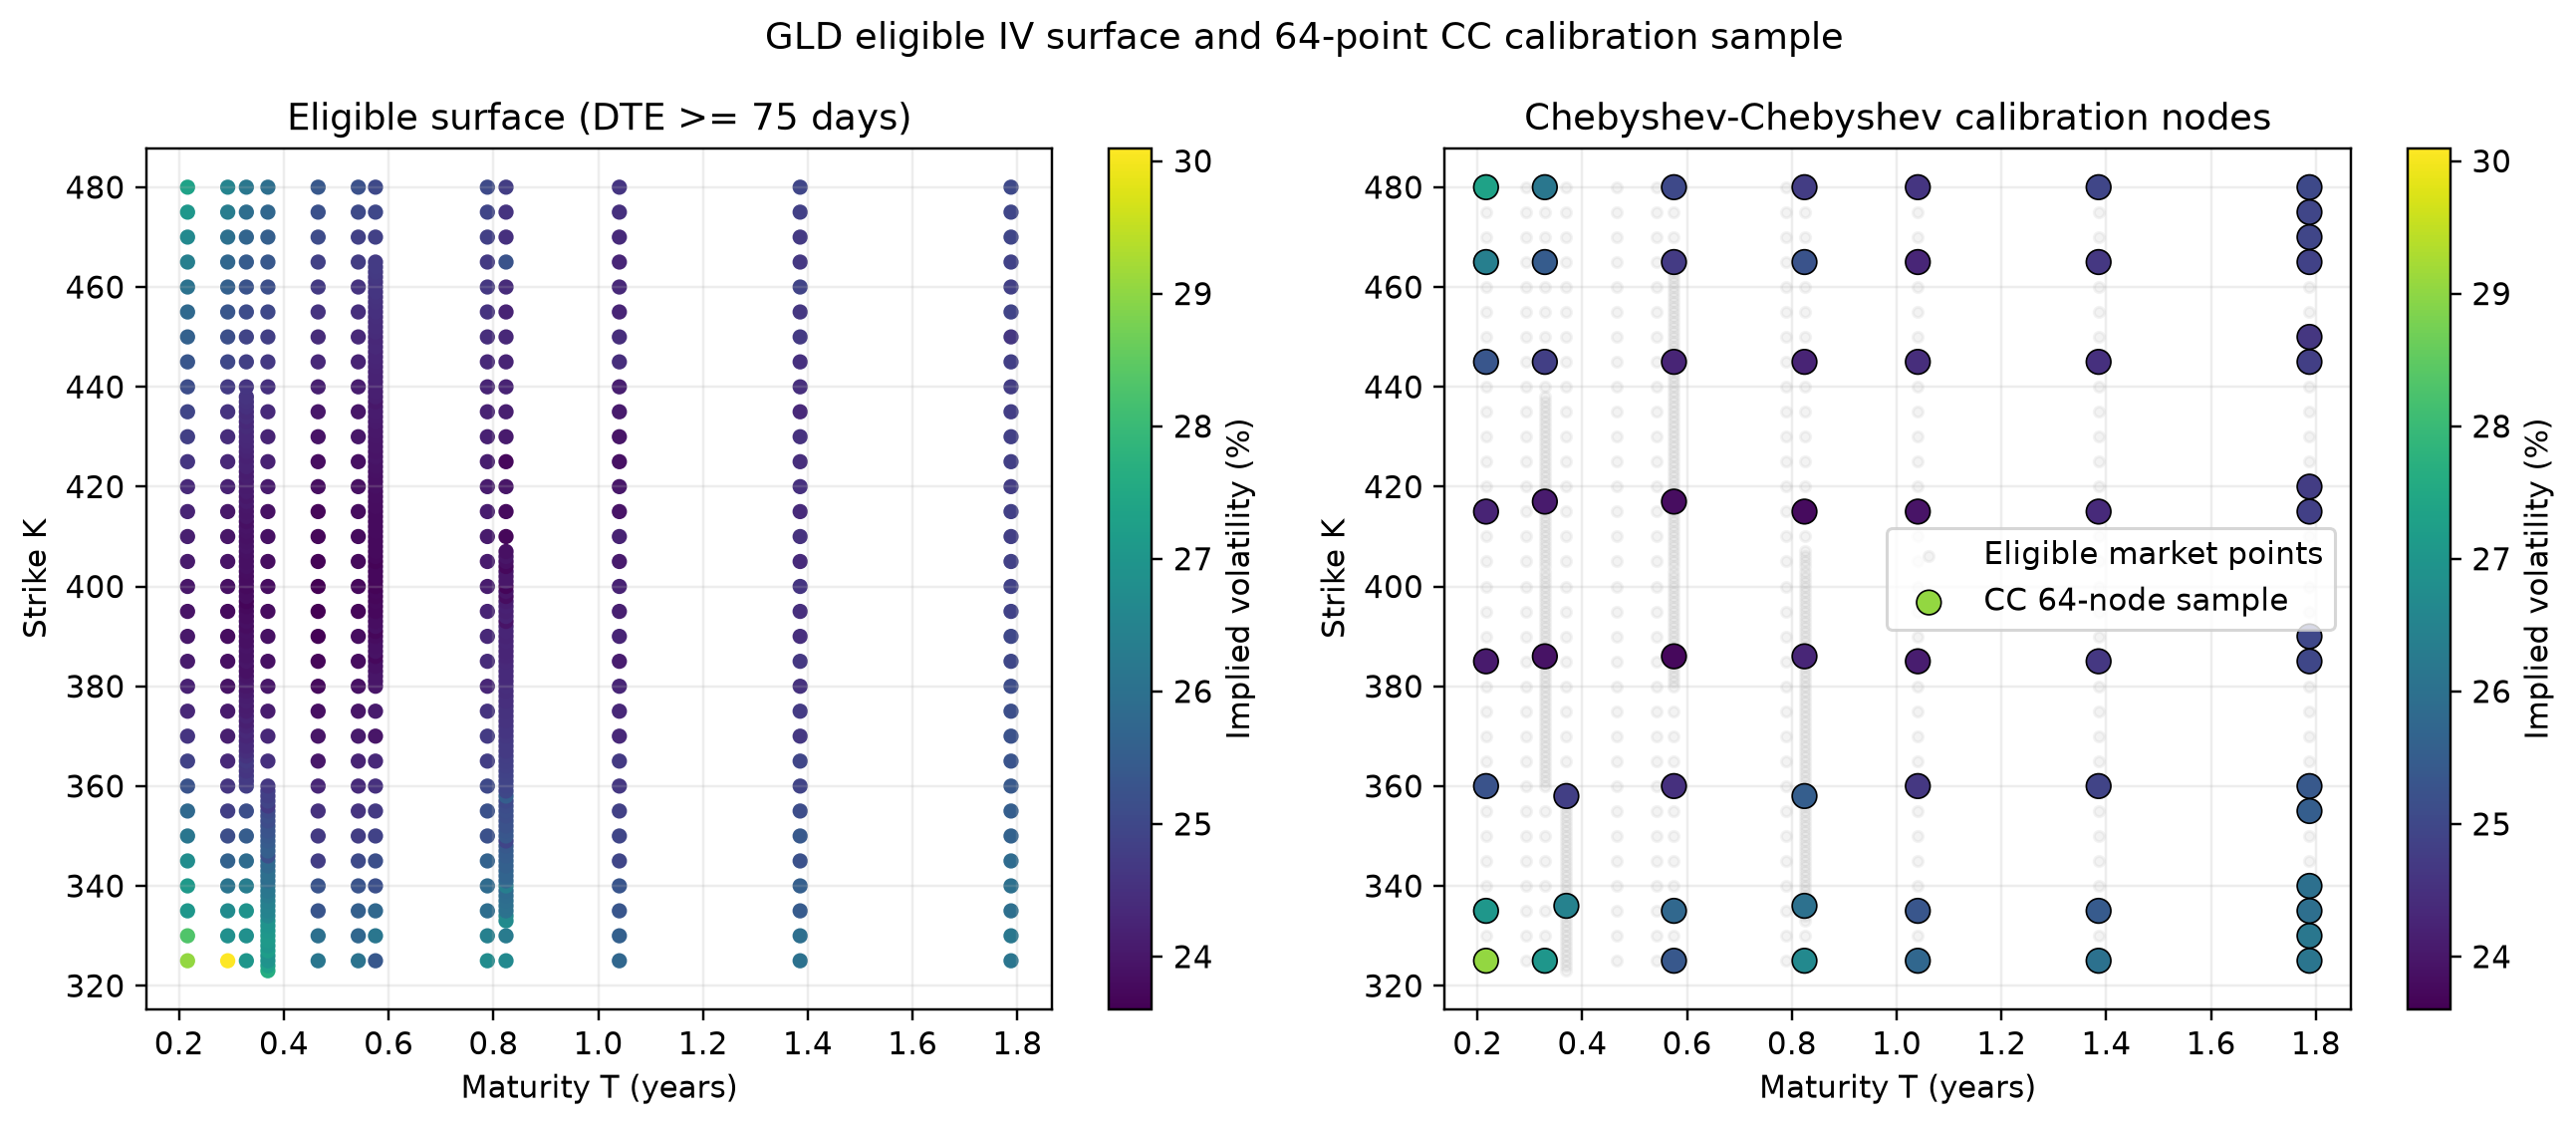
\includegraphics[width=0.88\textwidth]{../img/publication/571681dc4acfdf64_sampling_comparison.png}
    \caption{Team 8 calibration inputs. Top: 14 same-date continuously compounded U.S. Treasury proxies and their NSS fit
on 2 September 2026. Bottom: the CC64 sample selected from 605 eligible GLD calls
across 12 expiries and 146 strikes; the retained contracts span eight expiries
and 20 strikes. The colours encode observed
    implied volatility; the node layout, rather than an interpolated sheet,
    is the actual object passed to the optimizer.}
    \label{fig:t8-market-inputs}
\end{figure}

The historical GLD return series supplies a different diagnostic from the
option cross-section. It is observed under the historical data-generating
process and is used only to test Gaussian adequacy, not to estimate a physical
drift or to rank option-pricing models. Figure~\ref{fig:t8-return-normality}
shows both the central concentration and the tail departures that motivate a
variance-and-jump model stack.

\begin{figure}[H]
    \centering
    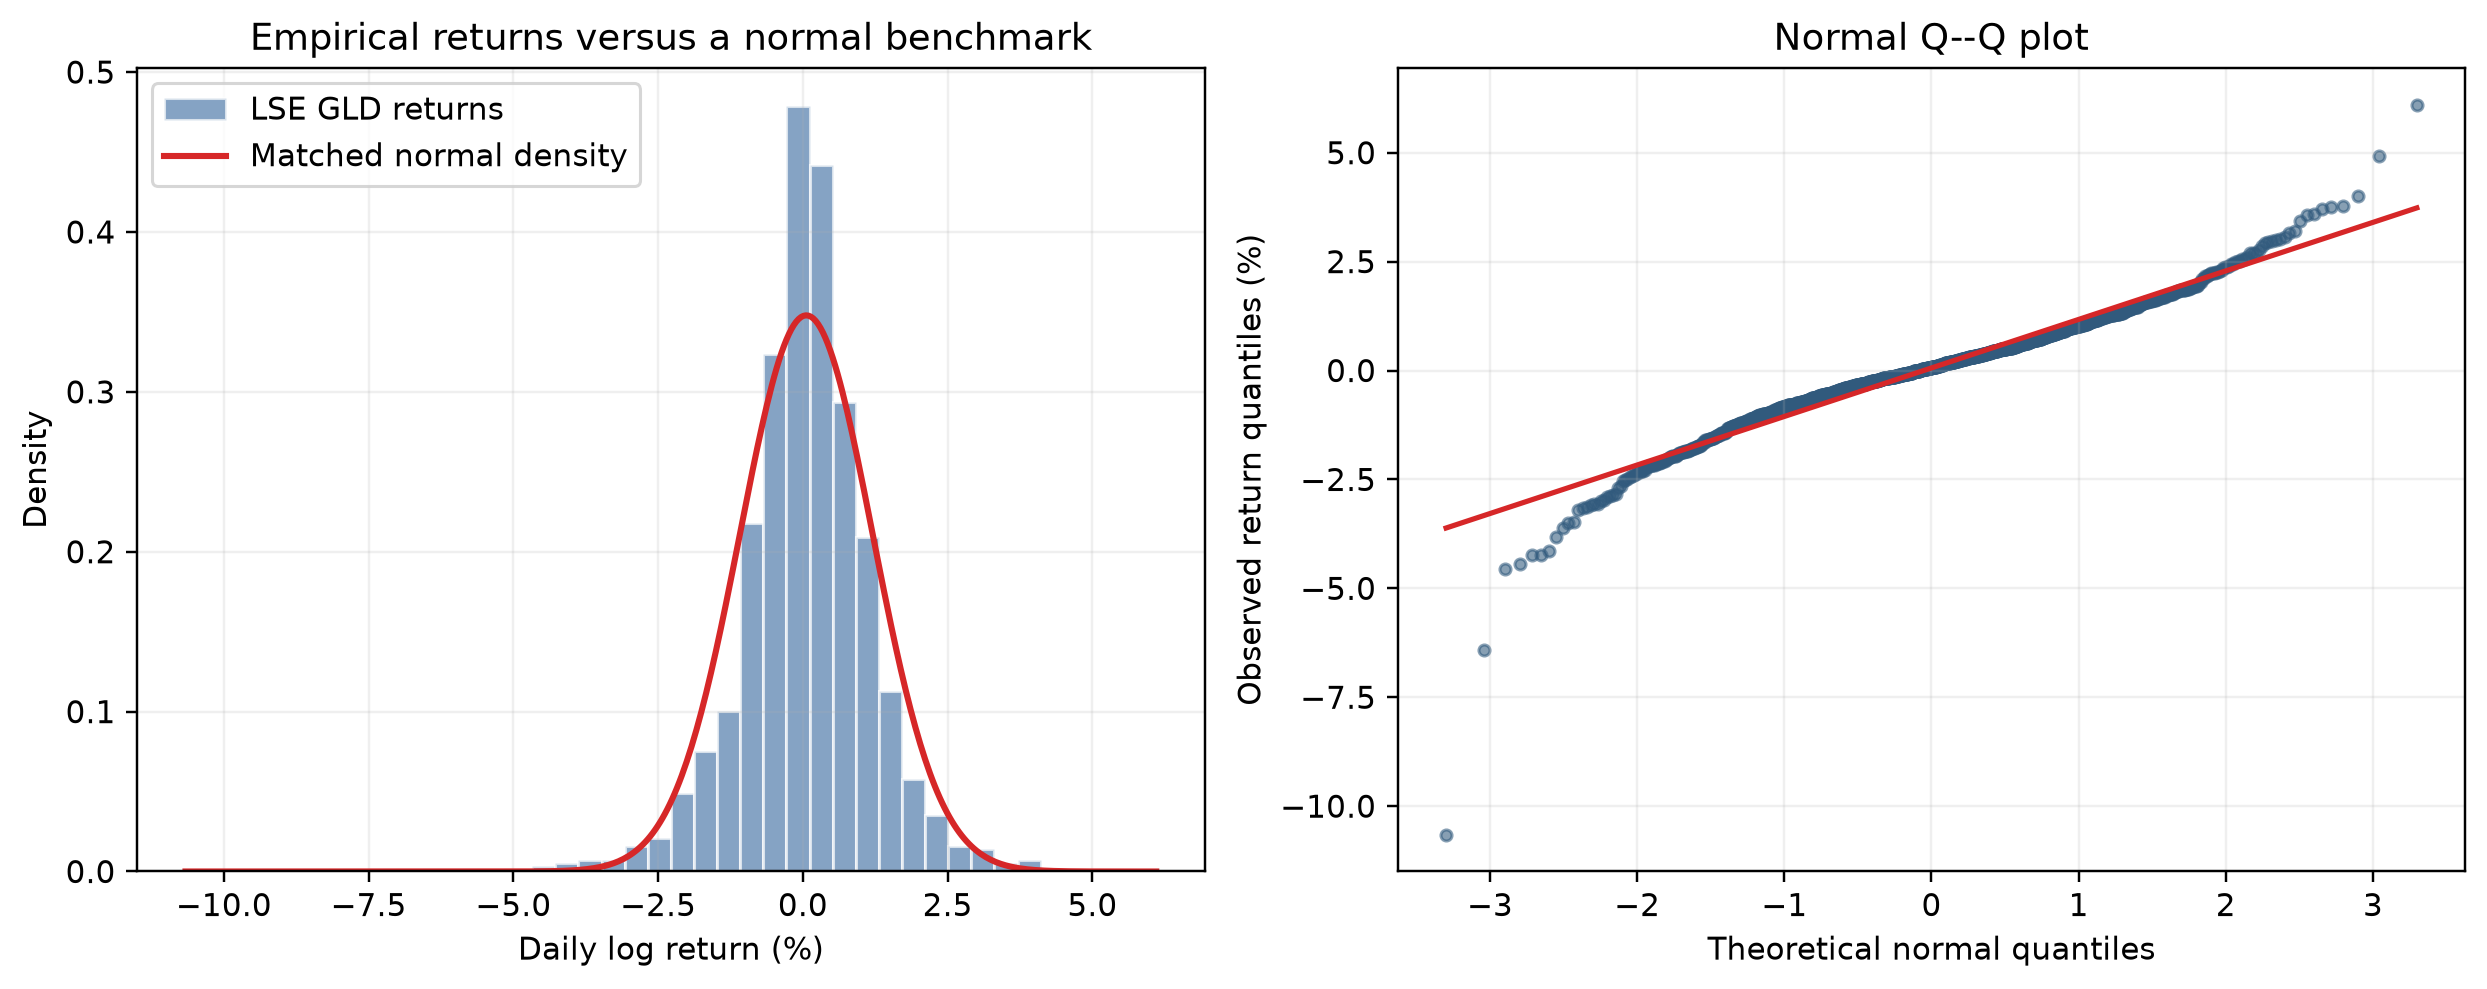
\includegraphics[width=0.96\textwidth]{../img/publication/c011553eac7f680d_gld_return_normality.png}
    \caption{LSE (London Strategic Edge) GLD daily log returns from 5 January 2021 to 27 August 2026:
    empirical density against a matched normal law and normal Q--Q plot. The
    sample contains 1,424 observations; the visible tail departures are
    consistent with the formal tests in Table~\ref{tab:t8-return-normality}.}
    \label{fig:t8-return-normality}
\end{figure}

\begin{table}[H]
\centering
\footnotesize
\begin{tabular}{@{}lrrl@{}}
\toprule
Test & Statistic & \(p\)-value & Decision at 5\% \\
\midrule
Shapiro--Wilk & 0.9434 & \(6.25\cdot10^{-23}\) & Reject normality \\
Jarque--Bera & 3499.31 & \(<10^{-300}\) & Reject normality \\
D'Agostino \(K^2\) & 322.83 & \(7.90\cdot10^{-71}\) & Reject normality \\
\bottomrule
\end{tabular}
\caption{Normality tests for the 1,424 daily GLD log returns. Sample skewness
is \(-0.733\) and excess kurtosis is \(7.570\). Rejection motivates richer
dynamics but does not by itself select Heston, Bates or Bates--Hawkes.}
\label{tab:t8-return-normality}
\end{table}

\subsubsection{Cross-sectional calibration geometry}

Tables~\ref{tab:t8-model-parameters}--\ref{tab:t8-model-errors} consolidate
the point-in-time fit that is otherwise distributed across the model-specific
sections. All four rows use the same 64 actual nodes, price/IV conversion and
vega-weighted objective, and the same GLD carry $q=0.40\%$ applied through
$C(S,K;q)=e^{-qT}C(S,Ke^{qT};0)$; richer models therefore change the state law
rather than the empirical target. The fits were rebuilt on 24 October 2026:
Bates is refined from the nested Heston point and Full Bates--Hawkes from the
nested Bates point, and the nested candidate is always retained.

\begin{table}[H]
\centering
\scriptsize
\setlength{\tabcolsep}{2.6pt}
\begin{tabularx}{\textwidth}{@{}>{\RaggedRight\arraybackslash}p{2.35cm}>{\RaggedRight\arraybackslash}X>{\RaggedRight\arraybackslash}p{2.75cm}@{}}
\toprule
Model & Calibrated parameters & Admissibility \\
\midrule
Black--Scholes & \(\sigma=0.25878\). & Positive volatility. \\
Heston & \(v_0=0.065187,\; \kappa=2.9279,\; \theta_v=0.072793,\; \xi=0.65193,\; \rho=-0.12956\). & Feller gap 0.0012574; not binding. \\
Bates--Poisson & \(v_0=0.052474,\; \kappa=3.3990,\; \theta_v=0.057570,\; \xi=0.62559,\; \rho=-0.34825,\; \lambda=1.7215,\; \mu_J=0.067765,\; \sigma_J=0.053981\). & Feller binds (gap \(9.4\cdot10^{-9}\)). \\
Full Bates--Hawkes & \(v_0=0.048212,\; \kappa=3.3984,\; \theta_v=0.058309,\; \xi=0.62954,\; \rho=-0.35861,\; \lambda_0=1.3793,\; \bar\lambda=0.28944,\; \eta=0.82476,\; \beta=10.266,\; \mu_J=0.047409,\; \sigma_J=0.096630\). & Feller binds (gap \(1.3\cdot10^{-8}\)); stationary $\eta<1$. \\
\bottomrule
\end{tabularx}
\caption{Feller-constrained parameters on the current 2 September 2026 Team 8
Chebyshev sample with $q=0.40\%$, five significant digits, from
\texttt{data/processed/team8/calibration\_q040\_audited\_20261024}. The
Bates--Hawkes optimizer reported a constraint warning at exit; the retained
point is the admissible candidate with the lowest loss, below the nested Bates
loss.}
\label{tab:t8-model-parameters}
\end{table}

\begin{table}[H]
\centering
\scriptsize
\setlength{\tabcolsep}{3.1pt}
\begin{tabularx}{\textwidth}{@{}>{\RaggedRight\arraybackslash}p{2.35cm}rrrr>{\RaggedRight\arraybackslash}X@{}}
\toprule
Model & Price MAE & Price RMSE & IV MAE bp & IV RMSE bp & Reading \\
\midrule
Black--Scholes & 1.066 & 1.265 & 103.86 & \CalBSIVRMSE & Constant-volatility benchmark. \\
Heston & 0.526 & 0.668 & 52.18 & \CalHIVRMSE & Nested start for Bates. \\
Bates--Poisson & 0.527 & 0.671 & 50.75 & \CalBIVRMSE & Refined from Heston. \\
Full Bates--Hawkes & 0.479 & 0.584 & 42.60 & \CalWIVRMSE & Refined from Bates. \\
\bottomrule
\end{tabularx}
\caption{Calibration errors on a common option sample with $q=0.40\%$; prices
in USD per GLD share. Price and IV MAE are taken from the Article~8 diagnostic
table \texttt{model\_error\_summary.csv} of the same calibration. Because the
fits are nested, each richer model fits at least as well as the model it
contains; this cross-sectional fit is not an out-of-sample ranking.}
\label{tab:t8-model-errors}
\end{table}

The Full Bates--Hawkes branching ratio is \HawkesBranching, below unity, with
a kernel half-life $\log 2/\beta$ of \HawkesHalfLifeDays{} days and a
stationary mean intensity of \HawkesMeanIntensity{} jumps a year. This
snapshot permits material self-excitation, but does not establish stable
identification across regimes. The lower in-sample error of the richer models
follows from the nesting; predictive performance is assessed separately on the
rolling panel (Table~\ref{tab:current-dense-oos}).

\begin{tcolorbox}[colback=white,colframe=sfblue,boxrule=0.5pt,arc=1mm,left=3mm,right=3mm,title={Calibration fragility}]
\small
The Feller condition is imposed as a hard constraint and binds at the optimum
for Bates and Bates--Hawkes; without it the Heston loss falls by
\FellerRelaxedLossRatio\%. The Heston loss changes by less than 3\% for
$\kappa$ between \KappaFlatLow{} and \KappaFlatHigh, so mean reversion is
weakly identified. With $q=0.40\%$ the Bates jump intensity is \BatesLambda{}
a year rather than zero, but jump and Hawkes parameters rest on 64 calls and
are not individually identified. The carry itself is supported by independent
evidence: COMEX gold futures against the synchronous spot imply a GLD yield of
\FuturesYieldLow--\FuturesYieldHigh\% at 0.5--0.8 years. With the fee as carry
the fit deteriorates: in the carry-sensitivity refit the Heston price RMSE
rises from USD~\CarryPriceRMSEZero{} at $q=0$ to \CarryPriceRMSEFee{} at
$q=0.40\%$, and the loss increases in every moneyness bucket. Call-only
surfaces cannot separate carry from skew, so the futures-implied fee is used
rather than a fitted carry.
\end{tcolorbox}

The residual maps in Figures~\ref{fig:t8-residual-atlas-diffusion} and
\ref{fig:t8-residual-atlas-jumps} restore the spatial information hidden by
one RMSE. The continuous colours are interpolation only inside the observed
node domain; the circles identify the observations. Their purpose is to show
where errors remain systematic across maturity and moneyness.

\begin{figure}[p]
    \centering
    \includegraphics[width=0.49\textwidth]{\FigBlackScholesResidualHeatmap}\hfill
    \includegraphics[width=0.49\textwidth]{\FigHestonResidualHeatmap}
    \caption{Implied-volatility residuals for the two diffusion
    specifications on the common 2 September CC64 sample with $q=0.40\%$:
    Black--Scholes (left) and Feller-constrained Heston (right). Blue denotes
    model IV above market IV and red model IV below market; all maps share one
    colour scale. Stochastic variance reduces the scalar loss but does not
    remove structured maturity--moneyness error.}
    \label{fig:t8-residual-atlas-diffusion}
\end{figure}

\begin{figure}[p]
    \centering
    \includegraphics[width=0.49\textwidth]{\FigBatesResidualHeatmap}\hfill
    \includegraphics[width=0.49\textwidth]{\FigBatesHawkesResidualHeatmap}
    \caption{Implied-volatility residuals after adding discontinuities, same
    sample, carry and colour scale: Bates--Poisson (left) and Full
    Bates--Hawkes (right). The nested Hawkes layer lowers the current scalar
    error, while visible clusters remain.}
    \label{fig:t8-residual-atlas-jumps}
\end{figure}

\begin{figure}[p]
    \centering
    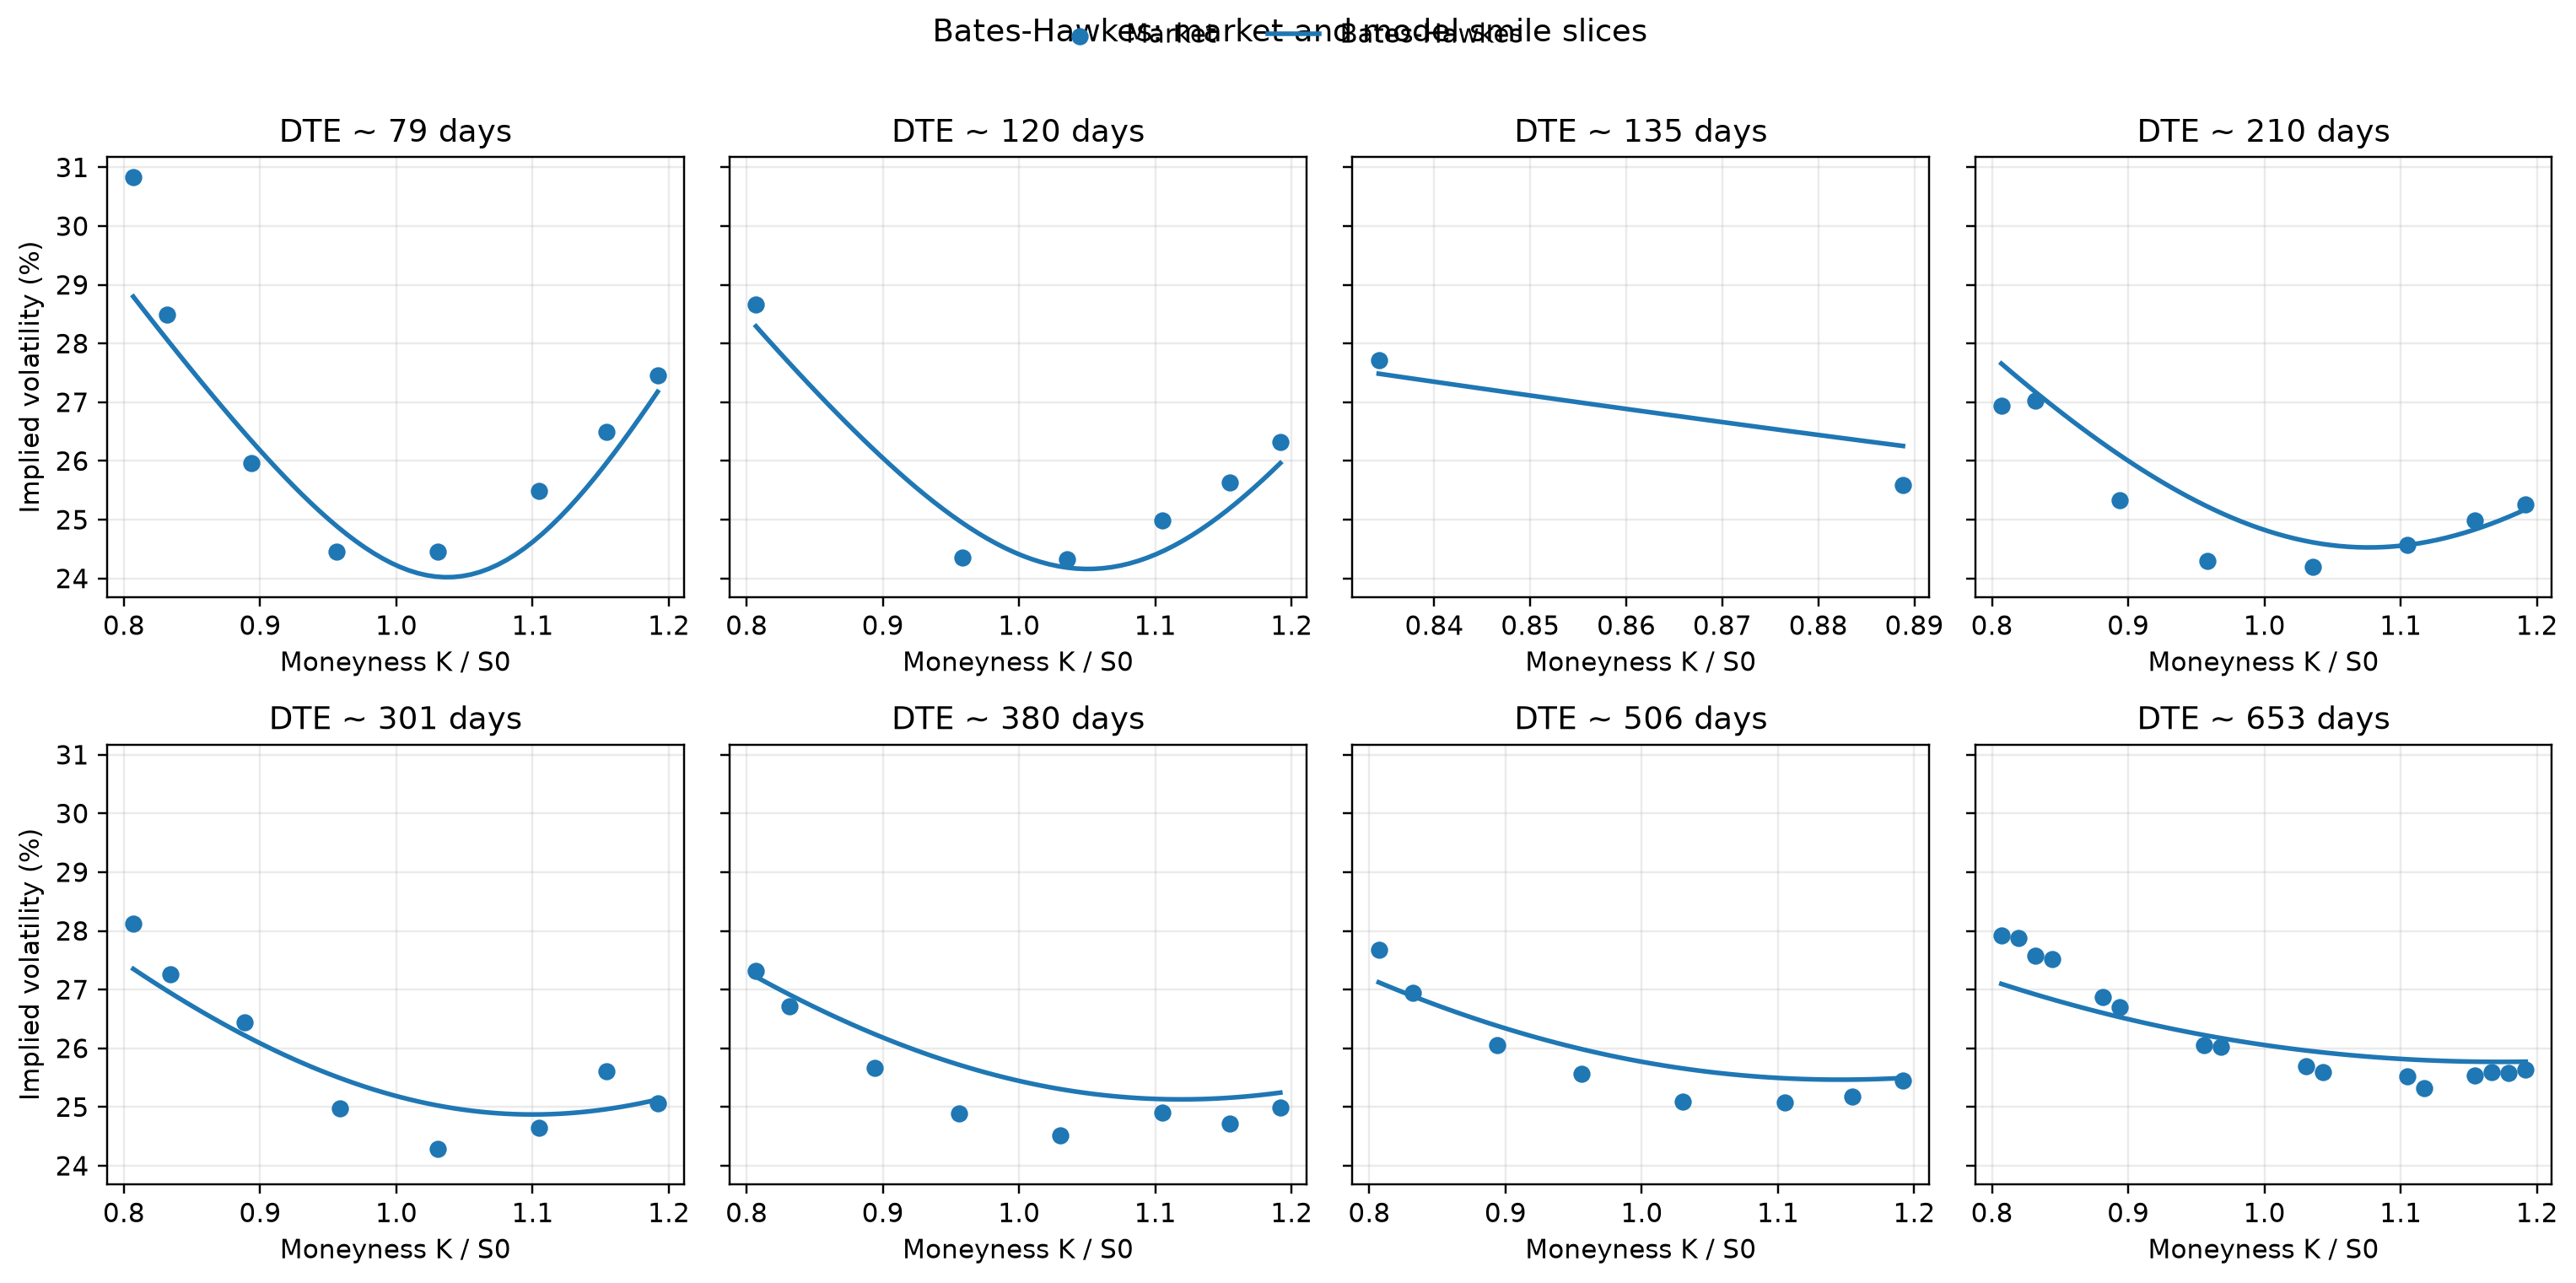
\includegraphics[width=0.97\textwidth]{../img/publication/0040f9f7c9958cde_bates_hawkes_volatility_smile.png}
    \caption{Observed and Full Bates--Hawkes implied-volatility smiles across
    the eight sampled expiries, regenerated from the $q=0.40\%$ calibration. The panel view prevents a low aggregate RMSE
    from concealing expiry-specific misses, especially at boundary strikes.}
    \label{fig:t8-bh-smiles}
\end{figure}

The standalone study also compared three Hawkes routes that estimate
different objects. Table~\ref{tab:t8-hawkes-routes} preserves that distinction:
event-time likelihoods are kernel diagnostics, whereas only an option-price
calibration can enter the like-for-like surface comparison.

\begin{table}[H]
\centering
\scriptsize
\setlength{\tabcolsep}{3pt}
\begin{tabularx}{\textwidth}{@{}p{2.25cm}p{2.55cm}p{3.45cm}X@{}}
\toprule
Route & Target & Source-study result & Role \\
\midrule
Exact constant-volatility Hawkes & GLD option surface & \(\sigma=0.22448\),
\(\eta=0.00460\), objective \(8.674\cdot10^{-5}\). & Transform benchmark;
excludes the Heston variance state. \\
Exponential kernel & Event times & \(\eta=0.3884\), log-likelihood \(-67.75\),
AIC 141.51, BIC 147.36. & Stable Markovian kernel compatible with affine
pricing. \\
Rough power-law kernel & Event times & \(\eta=0.4119\), log-likelihood \(-68.03\),
AIC 144.05, BIC 151.86. & Long-memory diagnostic; not the option-pricing
model used in the comparison. \\
\bottomrule
\end{tabularx}
\caption{Historical source-study Hawkes routes; these archived estimates are not the current September parameter set.}
\label{tab:t8-hawkes-routes}
\end{table}

\begin{figure}[p]
    \centering
    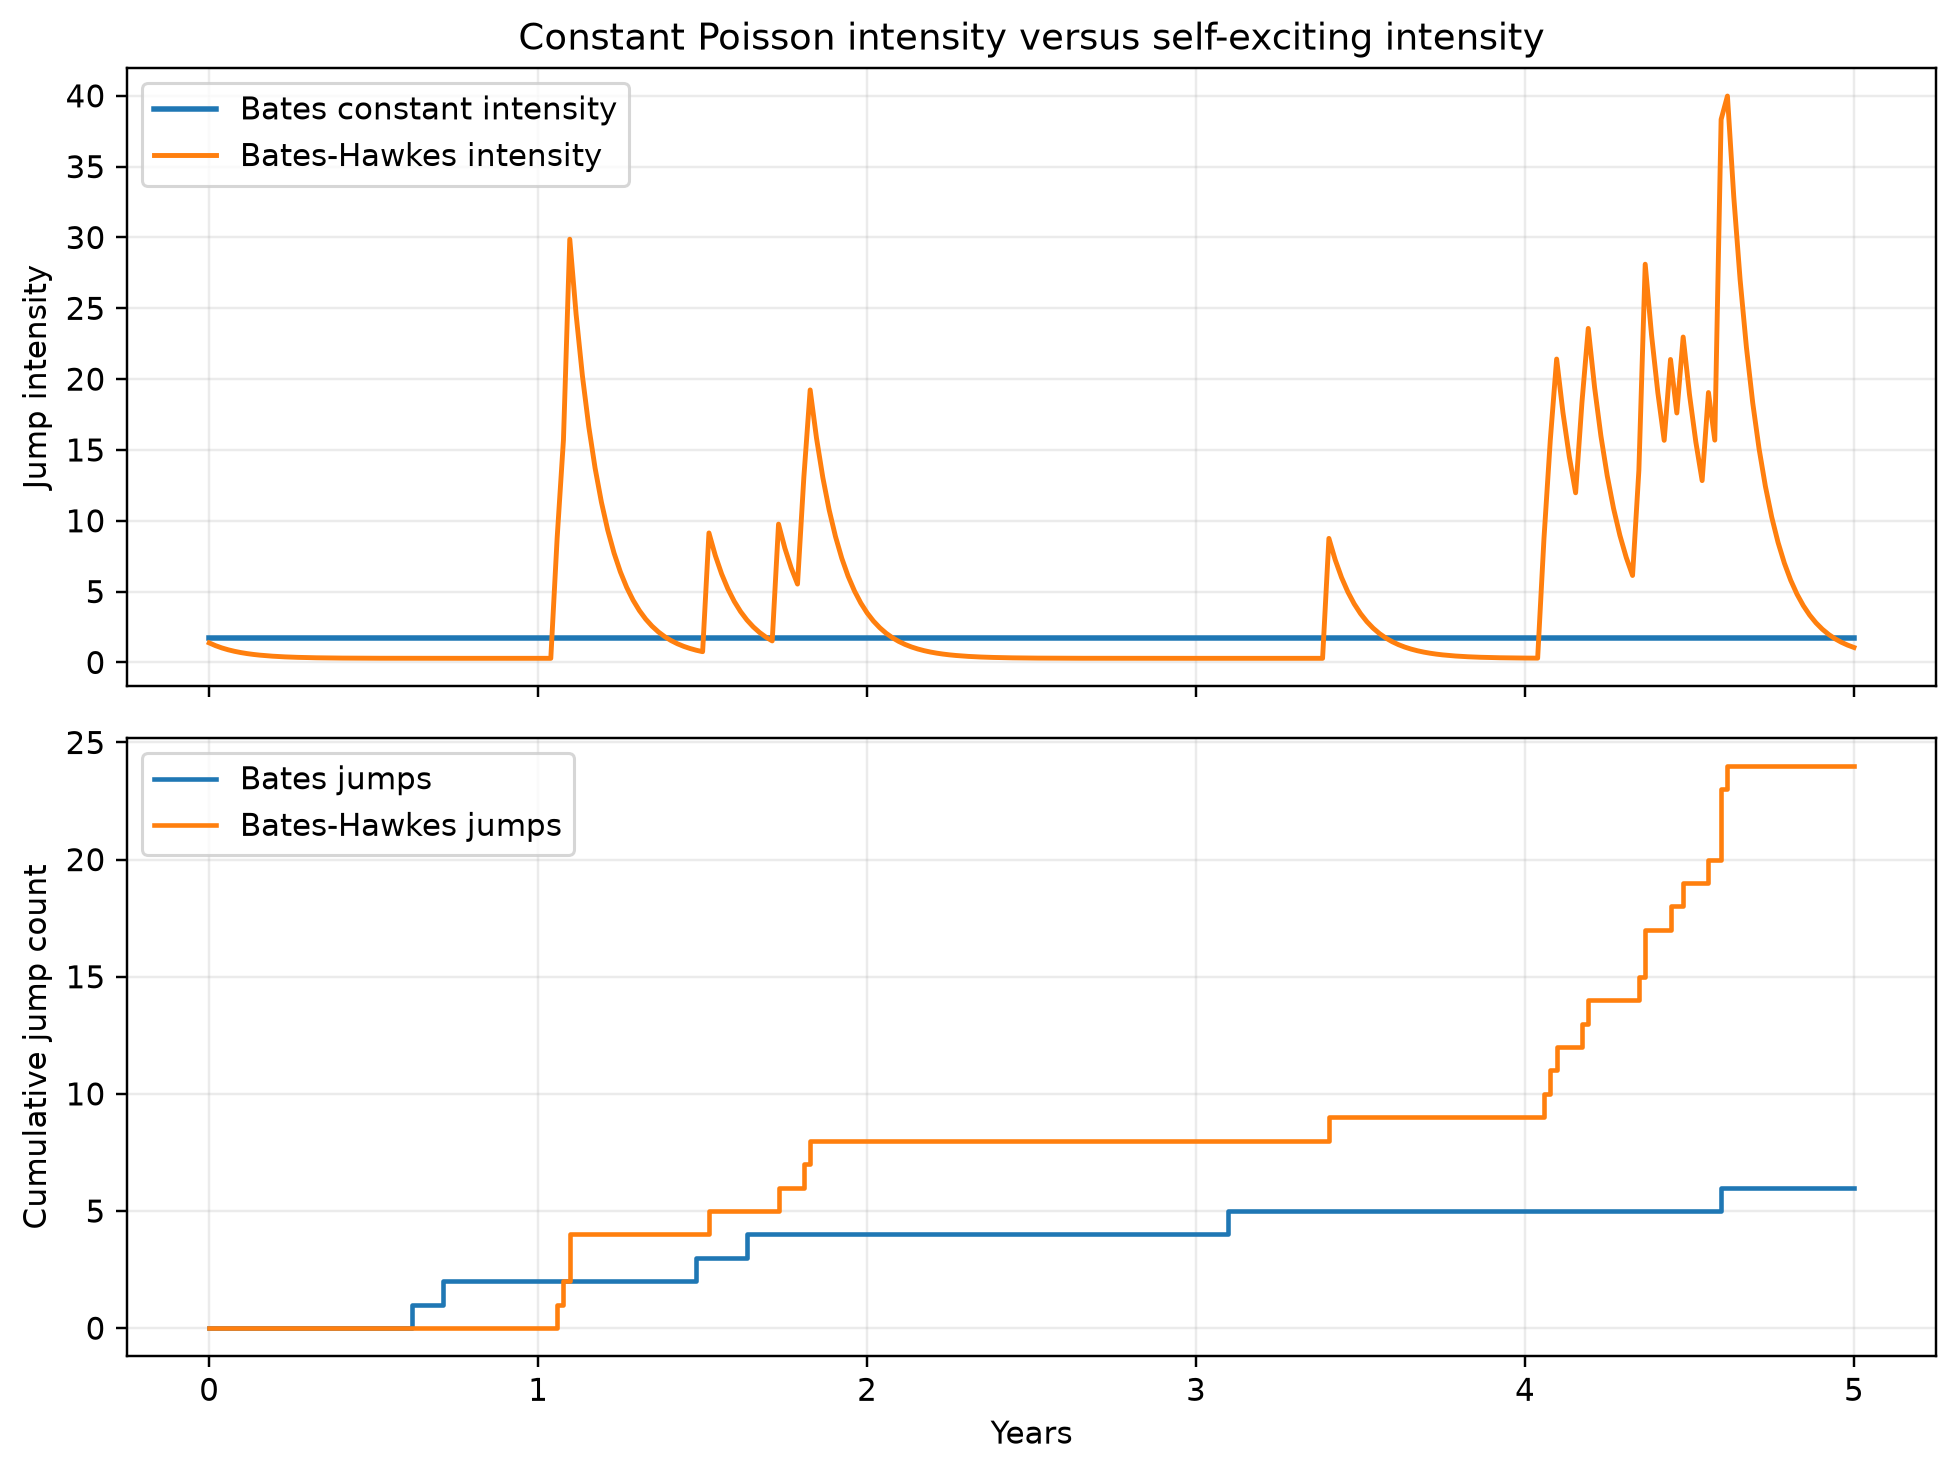
\includegraphics[width=0.94\textwidth]{../img/publication/c7008efadfbbd3d6_hawkes_intensity_comparison.png}
    \caption{Constant-intensity Bates jumps versus self-exciting
    Bates--Hawkes jumps regenerated from the current $q=0.40\%$ calibration
    with the corrected path engine. A Hawkes arrival raises
    near-term intensity, which subsequently decays toward its baseline; the
    lower panel shows the associated clustered event counts.}
    \label{fig:t8-hawkes-intensity}
\end{figure}

\begin{figure}[p]
    \centering
    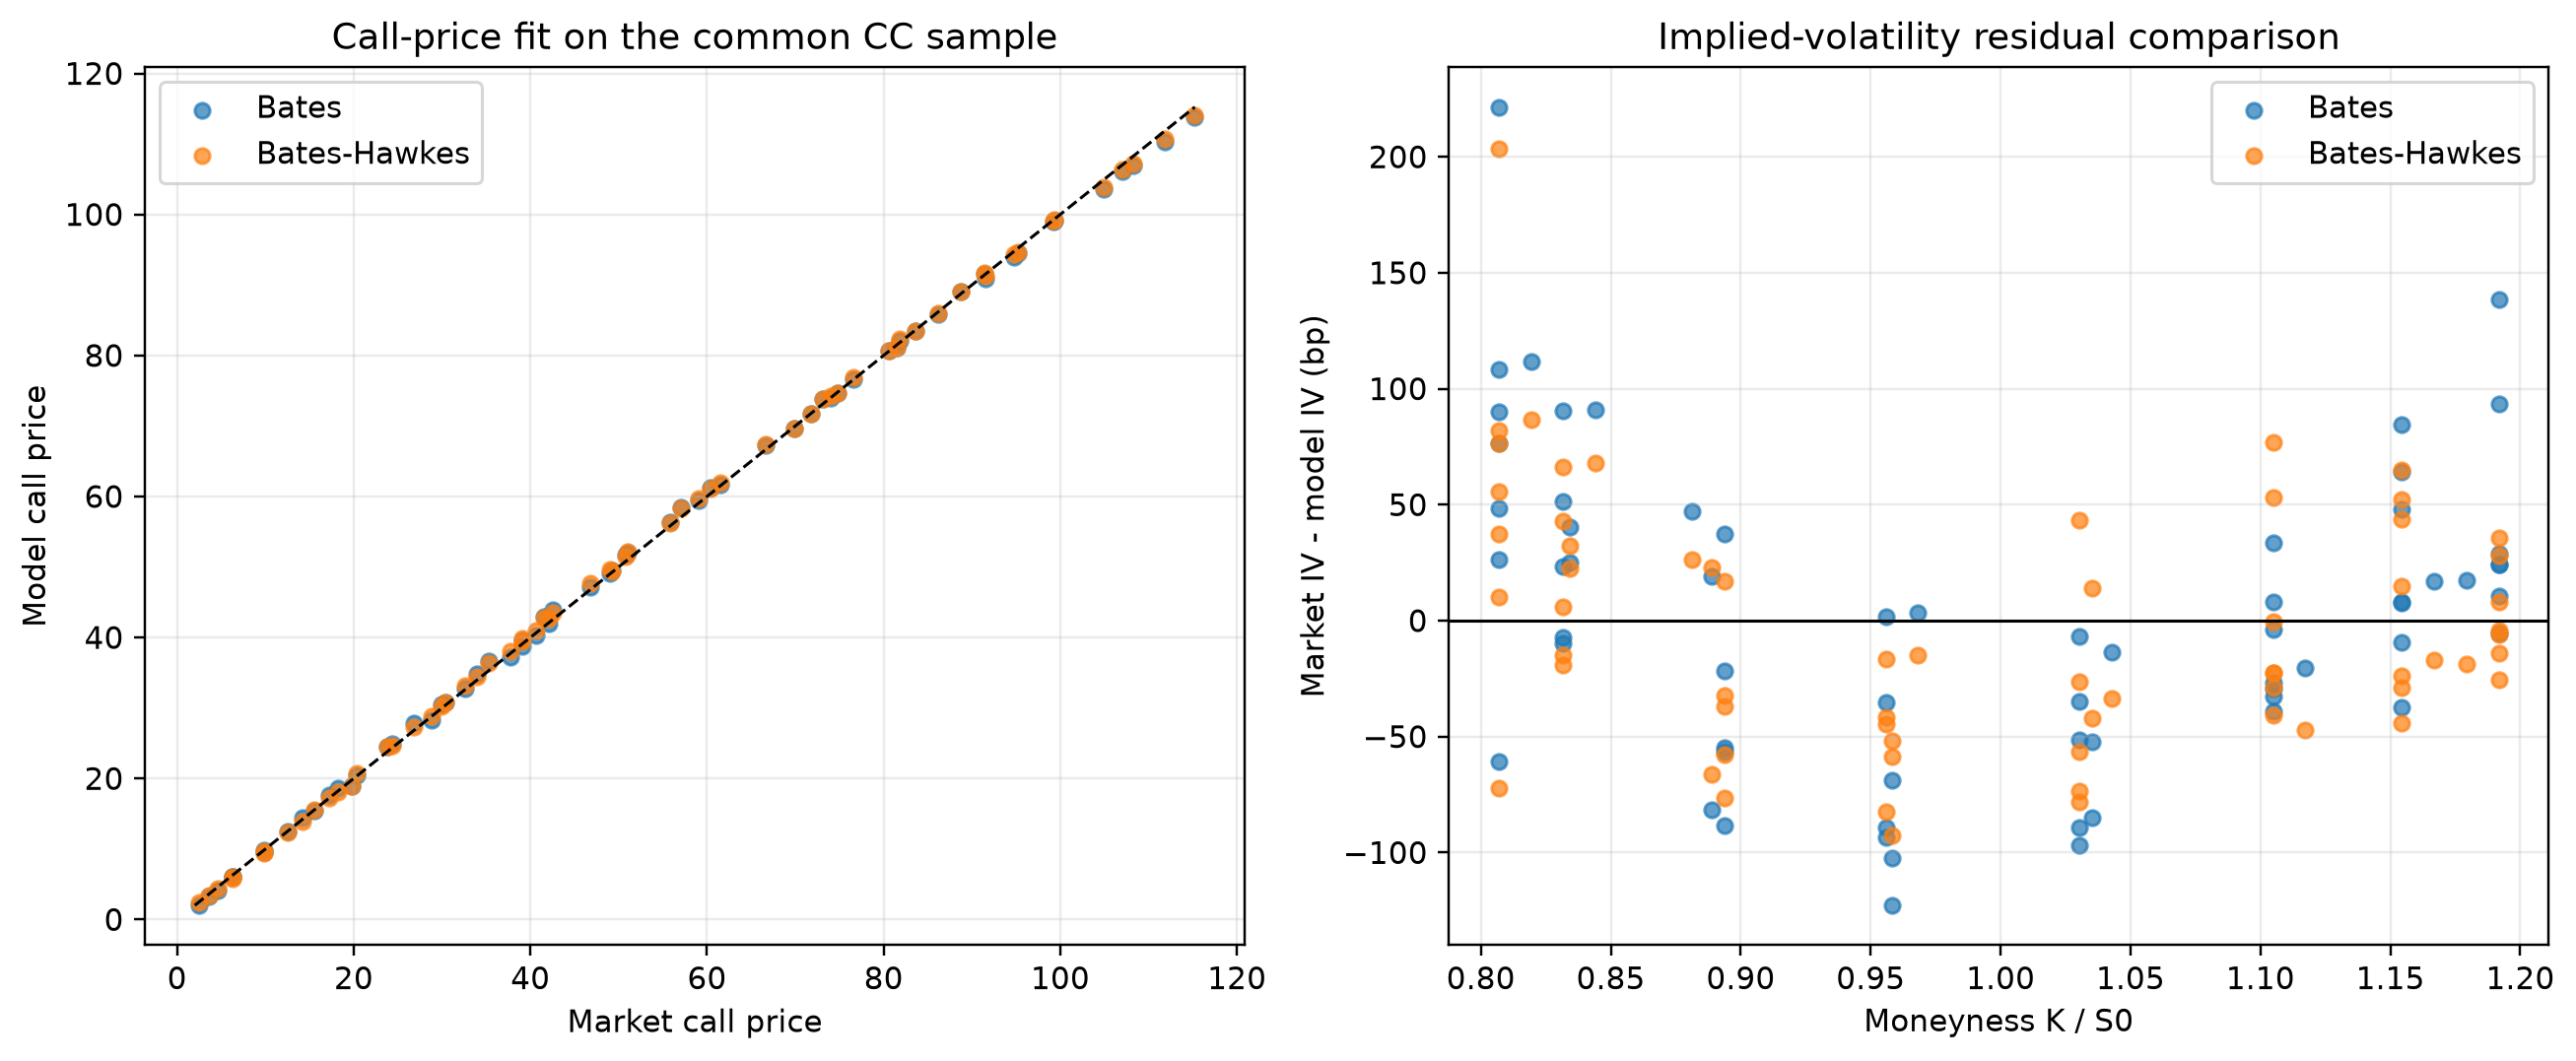
\includegraphics[width=0.98\textwidth]{../img/publication/82ef7fb46d8f7c23_bates_hawkes_vs_bates.png}
    \caption{Direct current-snapshot comparison between Full Bates--Hawkes and
    Bates--Poisson ($q=0.40\%$). The left panel checks option prices against the diagonal;
    the right panel compares market-minus-model IV residuals by maturity. This
    is cross-sectional fit evidence, not proof of predictive dominance.}
    \label{fig:t8-bh-versus-bates}
\end{figure}

\subsubsection{Chronological loss accumulation}

Figure~\ref{fig:t8-welch-goyal} summarises the rebuilt dense-only rolling
panel: \OosDates{} origins recalibrated with $q=0.40\%$ and equal optimizer
search for every model, scored on the next dense date. The benchmark is the
origin cross-sectional mean IV or the interpolated origin IV surface. Against
the mean the date-equal $R^2_{OOS}$ is $\OosBSRMean$, $\OosHRMean$,
$\OosBRMean$ and $\OosWRMean$\% for Black--Scholes, Heston, Bates and
Bates--Hawkes; against persistence it is $\OosBSRPersistence$,
$\OosHRPersistence$, $\OosBRPersistence$ and $\OosWRPersistence$\%, so no
model beats persistence; Black--Scholes does not even beat the mean.
Newey--West Diebold--Mariano tests of Bates--Hawkes against Black--Scholes,
Heston and Bates give $p$-values of \OosDMHawkesVsBSP, \OosDMHawkesVsHP{} and
\OosDMHawkesVsBP{} to three decimals, so its advantage over Bates is not
significant. These benchmark comparisons do not
establish physical gold forecasting accuracy.

\begin{figure}[p]
    \centering
    \includegraphics[width=0.80\textwidth]{\FigOosRmse}

    \vspace{3mm}
    \includegraphics[width=0.80\textwidth]{\FigOosRsquared}
    \caption{Dense-only rolling repricing with $q=0.40\%$ and equal optimizer
    search over \OosDates{} origins. Top: mean daily IV RMSE by model, with
    interpolated IV-surface persistence as the dashed reference. Bottom:
    date-equal $R^2_{OOS}$ against the origin mean IV and against persistence;
    positive values favour the model over the stated benchmark.}
    \label{fig:t8-welch-goyal}
\end{figure}
